\begin{frame}[allowframebreaks]{Signale}

    \begin{itemize}
        \item beschreiben, wie ein Parameter sich in Abhängigkeit eines anderen ändert
        \item x-Achse: Zeit/Frequenz
        \item y-Achse: Signalwert (abhängige Variable)
        \item Notation: $x[n]$ für diskrete Signale, Signalwert $x$ an Index $n$
    \end{itemize}
    \begin{figure}
        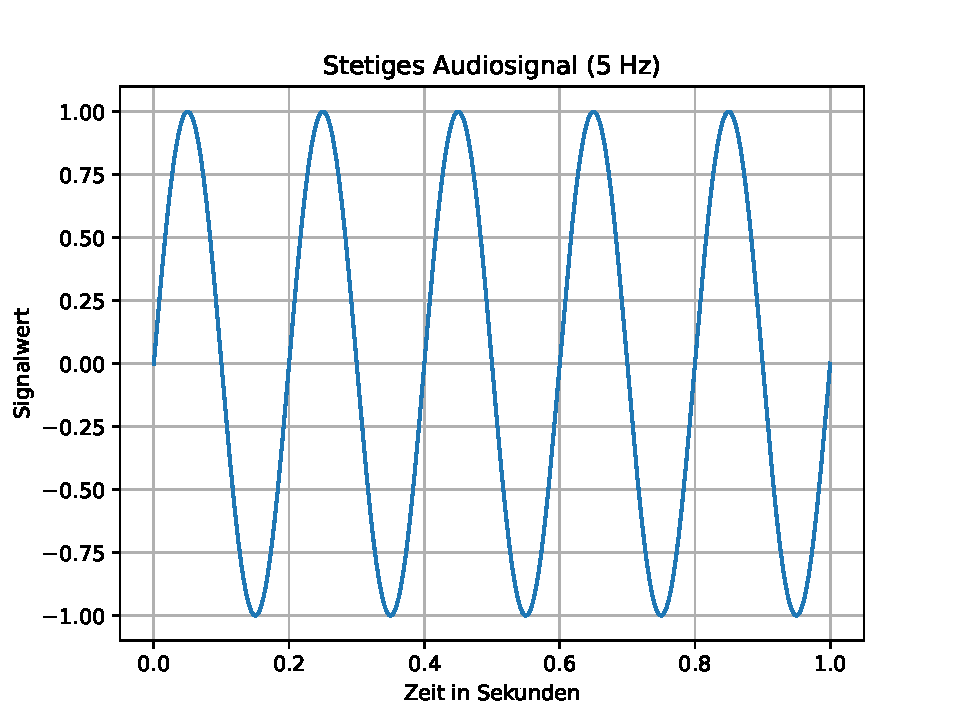
\includegraphics[width=0.6\textwidth]{Graphics/stetiges_signal.pdf}
    \end{figure}
        
    
\end{frame}

\begin{frame}[allowframebreaks]{Der Einheitsimpuls}
    \begin{itemize}
        \item Genauer: Einheits-Sample-Folge
    \end{itemize}

\begin{equation}
    \delta[n]=
    \begin{cases}
        0,\,n\ne0\\
        1,\,n=0
    \end{cases}
\end{equation}
    \begin{figure}
        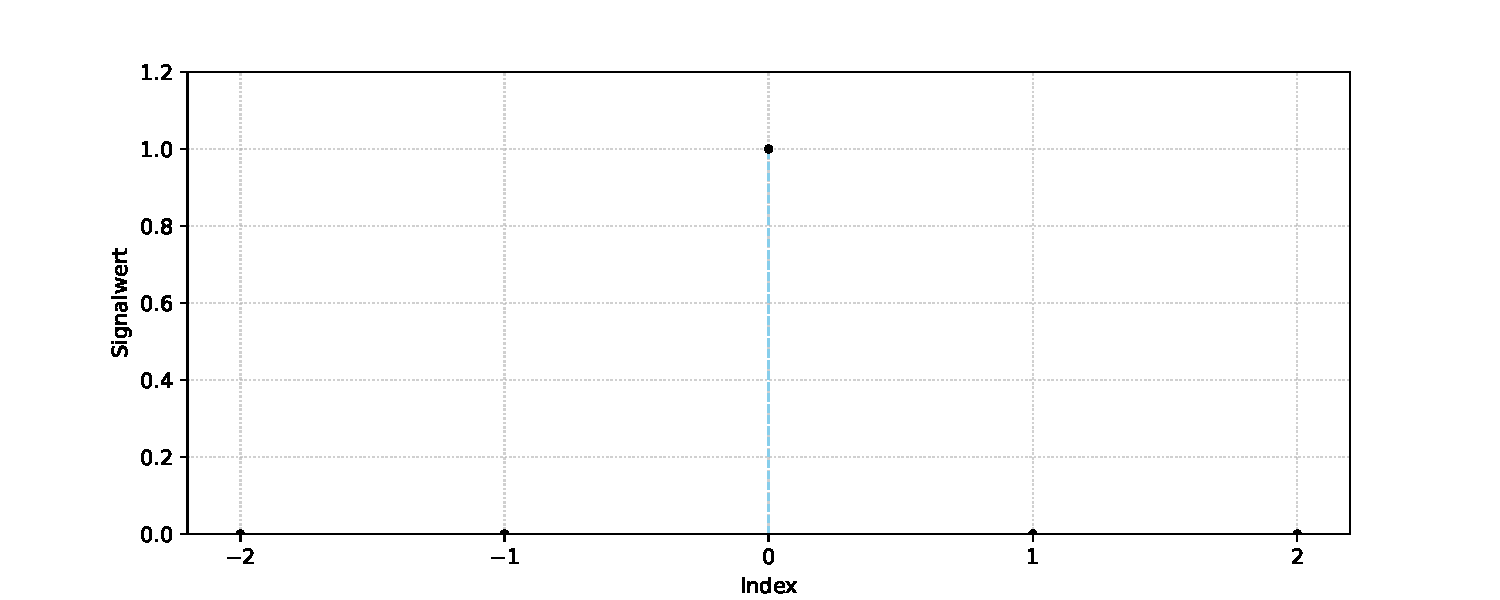
\includegraphics[width=0.8\textwidth]{Graphics/unitImpulse.pdf}
    \end{figure}

\end{frame}

\begin{frame}[allowframebreaks]{Systeme}
    \begin{itemize}
        \item System bildet Eingangssignal $x[n]$ auf Ausgangssignal $y[n]$ ab
        \item $T$: Transferfunktion des Systems
    \end{itemize}

    \[
        T:x[n]\mapsto y[n]
    \]
\end{frame}

\begin{frame}[allowframebreaks]{Lineare Zeit-Invariante Systeme}
    Lineare Systeme:
    \linebreak
    \begin{equation}
        T(x_1[n]+x_2[n])=T(x_1[n])+T(x_2[n])=y_1[n]+y_2[n]
    \end{equation}

    \begin{equation}
        T(a\cdot x[n])=a\cdot T(x[n])=a\cdot y[n]
    \end{equation}
    \begin{itemize}
        \item Summe der Ausgangssignale ist gleich Ausgangsignal bei vorheriger Summierung der Eingangssignale.
    \end{itemize}


    \framebreak

    Zeit-Invariante Systeme:
    \linebreak
    \begin{itemize}
        \item für jedes $n_0\in\mathbb{N}$ und jedes Eingangssignal $x[n]$ mit $x'[n]=x[n-n_0]$ wird das entsprechende Ausgangssignal $y$ mit $y'[n]=y[n-n_0]$ erzeugt.
        \item Verzögertes Eingangssignal $\rightarrow$ verzögertes, sonst gleiches, Ausgangssignal.
    \end{itemize}

    \framebreak

    Systeme mit beiden Eigenschaften: \textit{Lineare Zeit-Invariante Systeme}
    \linebreak
    \begin{itemize}
        \item Werden vollständig durch ihre Impulsantwort charakterisiert.
        \item Kurzschreibweise: LTI-System
    \end{itemize}

\end{frame}